% REMEMBER: Write the thesis from the view of the reader. How would I like to READ the thesis?
% WHY -> WHAT -> HOW structure

% 6th, 7th grade

\chapter{Evaluation}%
\label{cha:evaluation}

TODO: Introduction

- In this chapter, the Whisker testing utility is evaluated

- 3 Parts
- TODO: explain RQs
    - 1. First it is shown that it is possible to run Whisker tests without interfering with the execution of the Scratch program
    - 2. The main part of the evaluation focuses on finding out how accurate Whisker's test results can be compared to manual assessment (normal + constraint tests)
    - 3. Then Whiskers random input is evaluated

- Chapter outline

\section{Experimental Setup}

\subsection{Projects Under Test}

\subsubsection*{Catching Game}

=== Scratch Projects:
- From a students course
- Two groups, grade 6 and grade 7 $\rightarrow$ realistic for Whisker's purpose
- Multiple exercises to familiarize themselves with Scratch
- Build up to final, most complex, project
- Project has a clear and unambiguous description $\rightarrow$ well defined

=== Are these projects suitable for evaluating Whisker?
- Complexity on the higher end of what Whisker is supposed to be used for
- Game Over state makes it hard to assess other properties if the program goes game over because of a bug
    - E.g. one project would often go game over when an apple touches the borders on the sides
    - Well defined $\rightarrow$ tests can be written without looking at the projects (but often problematic, e.g. clones, inexact implementations)
- Students were not aware of the fact, that their projects would be subjected to automated assessment later
    - Students often deliberately changed their programs from the specification (e.g. different fall speeds, different messages)
    - In a real scenario (in which Whisker is used for grading) students would have the possibility to test their projects beforehand
    $\rightarrow$ see Chapter 2 - Advantages

=== Program description
- The projects implement a small catching game
- Apples and bananas fall from the top of the screen
- The player earns points by catching the fruit by moving a bowl with the left and right arrow keys
- If an apple touches the ground the game is over
- If a banana touches the ground point is subtracts points
- The game is over after 30 seconds elapsed

\begin{figure}[ht]
    \centering
    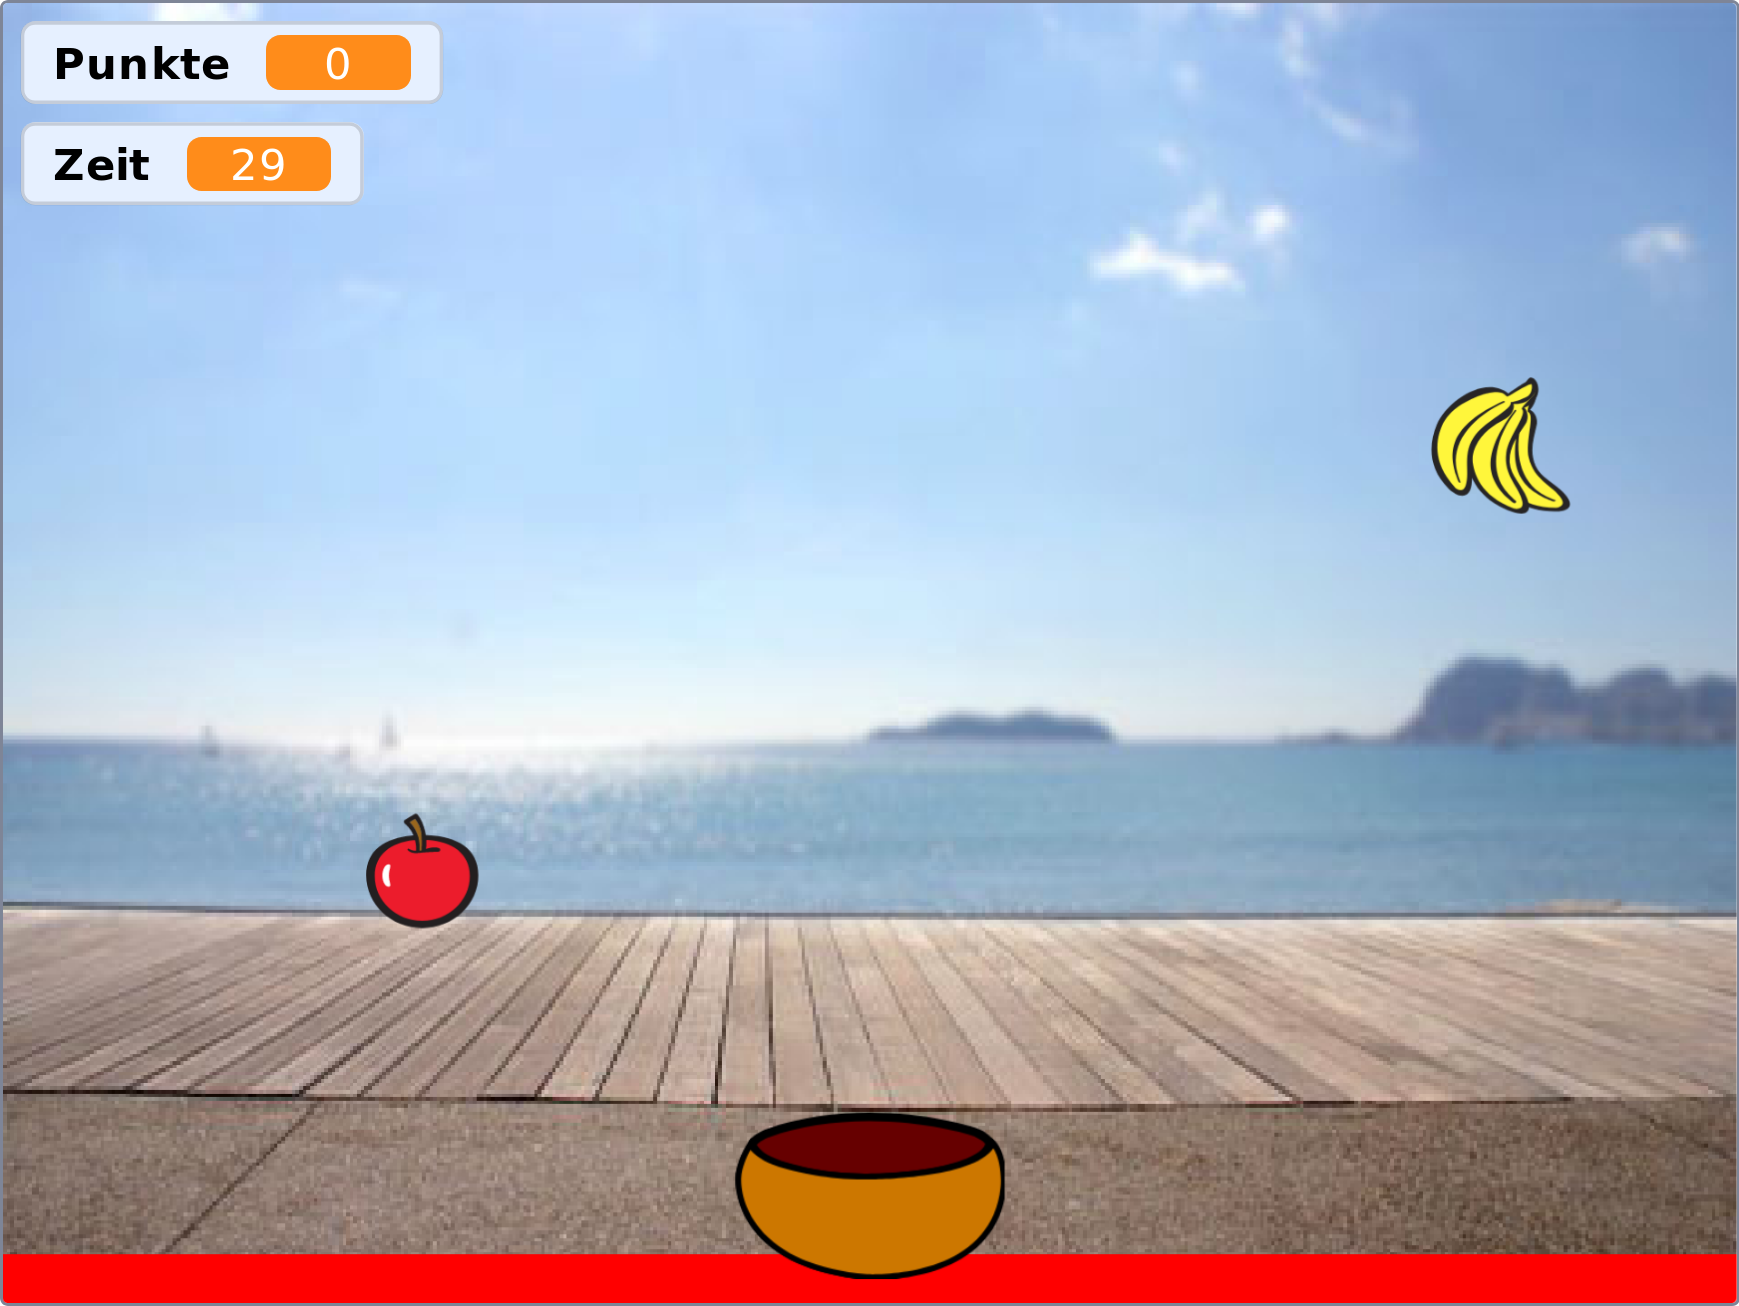
\includegraphics[width=0.35\textwidth]{scratch-stage}
    \caption{Screenshot of the sample solution}
    \label{fig:screenshot_of_the_sample_solution}
\end{figure}

- Table \ref{tab:project_specification} shows the full specification of the program as well as which of the test suites (ref ...) covers which parts of the specification.

=== Excluded Projects
- Some of the projects were excluded from the evaluation
- Because they where problematic to automated testing in some way
    - Tests select sprites and variables by name, and some projects changed the names of sprites and variables
        - Detected by searching the test reports: ''grep''
    - Some projects used a different mechanism than the green flag to start their program
        - Since this is not specified, tests can not start the program
        - Detected by zero statement coverage
    - Some Projects didn't work properly because of missing initialization
        - Go game over on startup
        - One project work if green flag is pressed multiple times
        - One project only worked if the sprites were manually dragged to a different position

\begin{table}
    \centering
    \scriptsize
    \begin{tabular}{ll}
        \toprule
        Project & Reason                                                                          \\
        \midrule
        \multicolumn{2}{l}{\textbf{Detected through the test report}}                             \\
        K6\_S12 & Deleted variable: time                                                          \\
        K6\_S17 & Renamed variable: "Punkte" to "Bunkte"                                          \\
        K7\_S24 & Deleted variable: time                                                          \\
        K7\_S27 & Renamed Sprite: "Bowl" to "Figur2"                                              \\[\medskipamount]

        \multicolumn{2}{l}{\textbf{Detected through zero statement coverage}}                     \\
        K6\_S01 & Starts on up key press instead of green flag                                    \\
        K6\_S06 & Wrong scratch project file (scored 30 points in manual rating but has no code)  \\
        K6\_S14 & Starts on space key press instead of green flag                                 \\[\medskipamount]

        \multicolumn{2}{l}{\textbf{Detected manually}}                                            \\
        K6\_S20 & Green flag has to be pressed twice to make it work properly                     \\
        K7\_S18 & Sprites have to be repositioned manually in the editor to make it work properly \\
        \bottomrule
    \end{tabular}
    \caption{Excluded projects}
    \label{tab:excluded_projects}
\end{table}

\subsubsection{Code Club Projects}

Code Club \cite{codeclub} offers free coding projects and step by step guide for programming beginners. (aimed towards children)
For each project, a sample solution is provided by a volunteer.
These projects will be used to measure the achieved coverage by automatically generated test input.
They are suited for this task, because
    - they are used for educational purposes
        $\rightarrow$ fits Whisker's purpose for automated grading
    - they are diverse
        $\rightarrow$ different kinds of programs and games

TODO: table?

\subsection{Test Suites}

\begin{table}
    \centering
    \scriptsize
    \begin{tabular}{lccc}
        \toprule
        Specification                                                                         & (1)    & (2)                   & (3)                   \\
        \midrule
        \textbf{Initialization} \\
        Timer starts at 30 seconds                                                            & \cmark & \xmark                & \xmark                \\
        Bowl starts at $X = 0$ / $Y = -145$                                                   & \cmark & \xmark                & \xmark                \\
        Fruits have a size of 50\%                                                            & \cmark & \cmark                & \cmark                \\[\medskipamount]
        \textbf{Bowl Movement} \\
        Bowl moves left/right when corresponding arrow key is pressed                         & \cmark & \cmark                & \cmark                \\
        Bowl can only move horizontally with a speed of 10                                    & \cmark & \cmark                & \cmark                \\[\medskipamount]
        \textbf{Fruit Falling} \\
        Apples fall down                                                                      & \cmark & \textasteriskcentered & \textasteriskcentered \\
        Apples fall in a straight line with a speed of -5                                     & \cmark & \cmark                & \cmark                \\
        Bananas fall down                                                                     & \cmark & \textasteriskcentered & \textasteriskcentered \\
        Bananas fall in a straight line with a speed of -7                                    & \cmark & \cmark                & \cmark                \\[\medskipamount]
        \textbf{Fruit Spawn} \\
        Apples spawn again at the top of the screen after touching the bowl                   & \cmark & \textasteriskcentered & \xmark                \\
        Apples spawn at random $X$ position                                                   & \cmark & \cmark                & \xmark                \\
        Apples spawn at $Y = 170$                                                             & \cmark & \cmark                & \xmark                \\
        Bananas spawn again at the top of the screen after touching the bowl                  & \cmark & \textasteriskcentered & \xmark                \\
        Bananas spawn at random $X$ position                                                  & \cmark & \cmark                & \xmark                \\
        Bananas spawn at $Y = 170$                                                            & \cmark & \cmark                & \xmark                \\
        Only one apple must fall down at a time                                               & \cmark & \cmark                & \xmark                \\
        Only one banana must fall down at a time                                              & \cmark & \cmark                & \xmark                \\
        Banana must wait for a second before falling down in the beginning                    & \cmark & \xmark                & \xmark                \\
        Banana must wait for a second before falling down after displaying the ''-8'' message & \cmark & \xmark                & \xmark                \\[\medskipamount]
        \textbf{Fruit Interaction} \\
        Apple gives 5 points when it touches the bowl                                         & \cmark & \cmark                & \cmark                \\
        Game over when the apple touches the ground                                           & \cmark & \textasteriskcentered & \cmark                \\
        Apple displays ''Game Over!'' message when it touches the ground                      & \cmark & \textasteriskcentered & \cmark                \\
        Banana gives 8 points when it touches the bowl                                        & \cmark & \cmark                & \cmark                \\
        Banana subtracts 8 points when it touches the ground                                  & \cmark & \cmark                & \cmark                \\
        Banana displays ''-8'' message when it touches the ground                             & \cmark & \cmark                & \cmark                \\[\medskipamount]
        \textbf{Timer} \\
        Timer ticks down                                                                      & \cmark & \cmark                & \cmark                \\
        Game is over when timer reaches 0                                                     & \cmark & \cmark                & \xmark                \\
        Bowl must display ''Ende!'' message when timer reaches 0                              & \cmark & \cmark                & \xmark                \\
        \bottomrule
    \end{tabular}
    \caption{Project specifications and their coverage by the test suites}
    \label{tab:project_specification}
\end{table}

\subsection{Testing Environment}

\begin{table}
    \centering
    \scriptsize \tt
    \begin{tabular}{ll}
        \toprule
        Whisker    & Whisker     1.0 \\
        Scratch VM & Scratch VM  0.2.0-prerelease.20181005173109 \\
        Browser    & Chrome      70.0.3538.110 (64-Bit) \\
        JavaScript & V8          7.0.276.40 \\
        OS         & Windows 8.1 Version 6.3 (Build 9600) \\
        CPU        & Intel Core i5 4670 (4 x  3.40 GHz) \\
        GPU        & Nvidia GeForce GTX 1080 \\
        RAM        & 8GB DDR3-1600 \\
        \bottomrule
    \end{tabular}
    \caption{Test setup}
    \label{tab:test_setup}
\end{table}

\section{RQ1: Interference with the Program Under Test}

Since the tests execute code between steps in a single threaded environment,
they could, in theory, interfere with the program by slowing down the step cycle.
This can make the program behave differently, because Scratch programs use absolute timings (TODO figure).

~\\~\\
\textbf{RQ1.} typical tests don't interfere with the execution of typical Scratch programs
$\rightarrow$ measure how long Scratch takes for a step (WORK\_TIME AND time to render)
$\rightarrow$ measure how long each operation in the Whisker step procedure takes (e.g. callbacks, sprites, constraints)
$\rightarrow$ Explain how the times are measured

TODO: explain why testing procedure might interfere with Scratch programs (absolute timings)
TODO: timing diagram and table of timings for real tests
TODO: example code for tests that interfere and their test data

~\\~\\
\paragraph{Null hypothesis ($H_0$)}
Additional computations for testing are to slow to be executed while the program is running and stretch out the average time a step takes.
\paragraph{Alternative hypothesis ($H_1$)}
Additional computations for testing can be fast enough to not affect the average step time.

\section{RQ2: Accuracy of Test Results}
% \subsection{Evaluation Method}
% \subsection{Data Selection}
% \subsection{Threats to Validity}

\textbf{RQ2.}
- Automatic testing can facilitate grading of Scratch assignments
    (1) test results (normal tests and constraint tests) match the results of manual evaluation
    (3) test results (normal tests and constraint tests) are consistent enough to be used for grading
        $\rightarrow$ Plot difference number of test passes per project
        $\rightarrow$ Check average difference

- Manual analysis is used as ground truth

TODO: explain why accuracy is evaluated in this way
    - attention to automated grading
TODO: discuss scatter and bar plots

~\\~\\
=== (1)
\paragraph{Null hypothesis ($H_0$)}
Test results have no strong relation to the scores that were given to the projects manually.
\paragraph{Alternative hypothesis ($H_1$)}
The results of automated tests closely match the results of manual scoring.

~\\~\\
=== (2)
\paragraph{Null hypothesis ($H_0$)}
Automated test results show very different results each run and are thus not accurate enough to use them for grading.
\paragraph{Alternative hypothesis ($H_1$)}
Test results are consistent enough over multiple runs to provide accurate information for grading.

\section{RQ3: Testing with Random Inputs}

\textbf{RQ3.}
- The testing process can be done entirely in the background independent of testing scenarios (?)
    $\rightarrow$ Random input can be used for the test
    $\rightarrow$ The test can involve the user using the program like they normally would

% - Constraint Tests
%     - Different approach: One test executes the program only once and checks defined constraints in the background, see Section \ref{sec:constraint_only_tests}
%     - Deliberately control the bowl to win the game
%     - faster, but can be less accurate (show difference of average runtime)
%     - not everything in this project can be tested in a single run
%     - Better for quickly checking the program
%     - Example of a constraint test (or put it somewhere else?)
%     - Can be used with different sources of input (manual / simulated / random)
%     - Instead of passing tests, passing constraints are measured
%     - Tests with wrong sprite names are completely excluded in the evaluation

- Automatic test input generation
- Same constraints as the constraint tests vs. only constraints that can hold in the first few seconds every time
    - Random input instead of deliberately controlling the bowl
    - Useful to test the stability of the program (like Android Monkey \cite{androidmonkey})
    - The catching game is not well suited for this approach since random input will quickly result in a game over

TODO: discuss test results
TODO: discuss coverage results


\section{Threats to validity}
- Students often deliberately changed their programs from the specification (e.g. different fall speeds)
    - Tests were adjusted to allow a little more than the specification (e.g. different message)

- For each tests suite, many / all projects were executed in a row
    - Could have a performance impact (?), but Scratch doesn't need a lot of resources
    - If anything, it could have a negative impact on the results, but results are very positive

- Tests could interfere with the program under test (see prev. section)
    - But Scratch programs don't usually do calculations without moving any sprite
    - Most time related functionality is based on absolute time, slow-down would not affect it

- Browser JavaScript could be problematic

% \begin{figure}
%     \centering
%     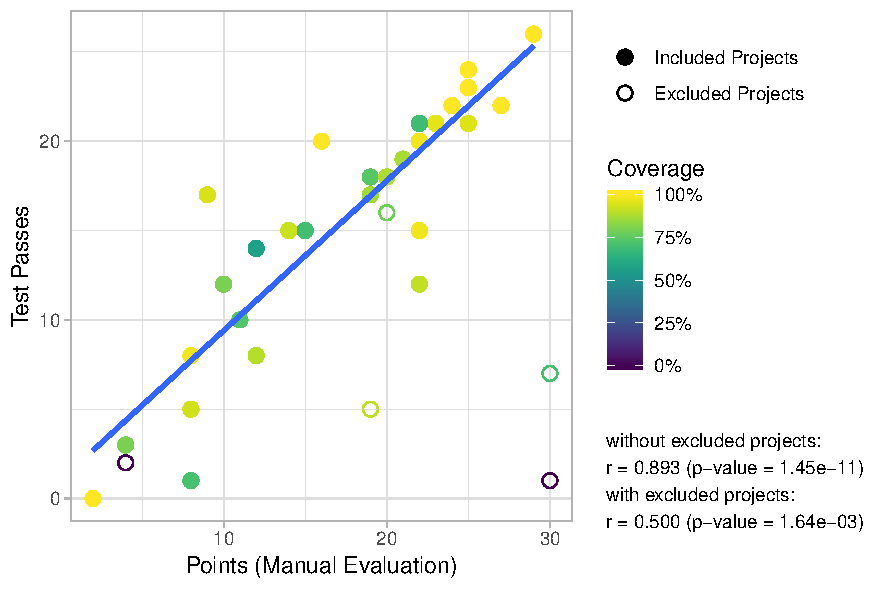
\includegraphics[width=.65\textwidth]{scatter-normal-1}
%     \caption{Results of the normal test suite (1)}
%     \label{fig:scatter_normal_1}
% \end{figure}
%
% \begin{figure}
%     \centering
%     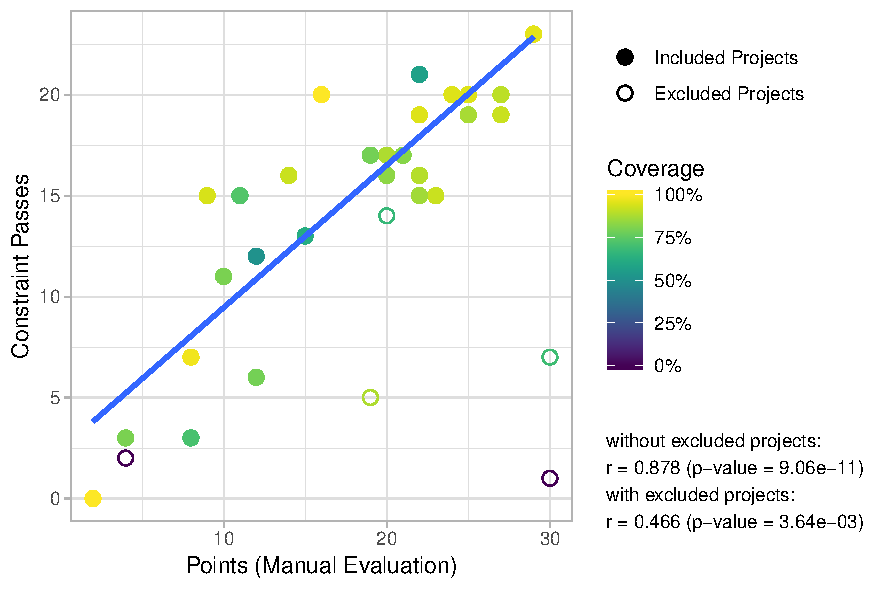
\includegraphics[width=.65\textwidth]{scatter-constraint-1}
%     \caption{Results of the constraint test suite (2) \\ with deliberately simulated input}
%     \label{fig:scatter_constraint_1}
% \end{figure}
